\documentclass{article}

\usepackage{fancyhdr}
\usepackage{extramarks}
\usepackage{amsmath}
\usepackage{amsthm}
\usepackage{amsfonts}
\usepackage{tikz}
\usepackage[plain]{algorithm}
\usepackage{algpseudocode}
\usepackage{listings} 
\usepackage{neuralnetwork}
\usepackage{subfigure}
\usetikzlibrary{automata,positioning}

\usepackage{color}

\definecolor{dkgreen}{rgb}{0,0.6,0}
\definecolor{gray}{rgb}{0.5,0.5,0.5}
\definecolor{mauve}{rgb}{0.58,0,0.82}

\lstset{frame=tb,
  language=Python,
  aboveskip=3mm,
  belowskip=3mm,
  showstringspaces=false,
  columns=flexible,
  basicstyle={\small\ttfamily},
  numbers=none,
  numberstyle=\tiny\color{gray},
  keywordstyle=\color{blue},
  commentstyle=\color{dkgreen},
  stringstyle=\color{mauve},
  breaklines=true,
  breakatwhitespace=true,
  tabsize=3
}
%
% Basic Document Settings
%

\topmargin=-0.45in
\evensidemargin=0in
\oddsidemargin=0in
\textwidth=6.5in
\textheight=9.0in
\headsep=0.25in

\linespread{1.1}

\pagestyle{fancy}
\lhead{\hmwkAuthorName}
\chead{\hmwkClass\: \hmwkTitle}
\rhead{\firstxmark}
\lfoot{\lastxmark}
\cfoot{\thepage}

\renewcommand\headrulewidth{0.4pt}
\renewcommand\footrulewidth{0.4pt}

\setlength\parindent{0pt}

%
% Create Problem Sections
%

\newcommand{\enterProblemHeader}[1]{
    \nobreak\extramarks{}{Task \arabic{#1} continued on next page\ldots}\nobreak{}
    \nobreak\extramarks{Task \arabic{#1} (continued)}{Problem \arabic{#1} continued on next page\ldots}\nobreak{}
}

\newcommand{\exitProblemHeader}[1]{
    \nobreak\extramarks{Task \arabic{#1} (continued)}{Problem \arabic{#1} continued on next page\ldots}\nobreak{}
    \stepcounter{#1}
    \nobreak\extramarks{Task \arabic{#1}}{}\nobreak{}
}

\setcounter{secnumdepth}{0}
\newcounter{partCounter}
\newcounter{homeworkProblemCounter}
\setcounter{homeworkProblemCounter}{1}
\nobreak\extramarks{Task \arabic{homeworkProblemCounter}}{}\nobreak{}

%
% Homework Problem Environment
%
% This environment takes an optional argument. When given, it will adjust the
% problem counter. This is useful for when the problems given for your
% assignment aren't sequential. See the last 3 problems of this template for an
% example.
%
\newenvironment{homeworkProblem}[1][-1]{
    \ifnum#1>0
        \setcounter{homeworkProblemCounter}{#1}
    \fi
    \section{Task \arabic{homeworkProblemCounter}}
    \setcounter{partCounter}{1}
    \enterProblemHeader{homeworkProblemCounter}
}{
    \exitProblemHeader{homeworkProblemCounter}
}

%
% Homework Details
%   - Title
%   - Due date
%   - Class
%   - Section/Time
%   - Instructor
%   - Author
%

\newcommand{\hmwkTitle}{Assignment\ \#1}
\newcommand{\hmwkDueDate}{March 10, 2019}
\newcommand{\hmwkClass}{CSCI964 Computational Intelligence}
\newcommand{\hmwkClassTime}{2.14}
\newcommand{\hmwkClassInstructor}{Zhifeng Wang}
\newcommand{\hmwkAuthorName}{\textbf{Mei Wangzhihui}}
\newcommand{\hmwkAuthorNum}{\textbf{2019124044}}
%
% Title Page
%

\title{
    \vspace{2in}
    \textmd{\textbf{\hmwkClass:\ \hmwkTitle}}\\
    % \normalsize\vspace{0.1in}\small{Due\ on\ \hmwkDueDate\ at 3:10pm}\\
    % \vspace{0.1in}\large{\textit{\hmwkClassInstructor\ \hmwkClassTime}}
    \vspace{3in}
}

\author{\hmwkAuthorName\ \hmwkAuthorNum}
\date{}

\renewcommand{\part}[1]{\textbf{\large Part \Alph{partCounter}}\stepcounter{partCounter}\\}

%
% Various Helper Commands
%

% Useful for algorithms
\newcommand{\alg}[1]{\textsc{\bfseries \footnotesize #1}}

% For derivatives
\newcommand{\deriv}[1]{\frac{\mathrm{d}}{\mathrm{d}x} (#1)}

% For partial derivatives
\newcommand{\pderiv}[2]{\frac{\partial}{\partial #1} (#2)}

% Integral dx
\newcommand{\dx}{\mathrm{d}x}

% Alias for the Solution section header
\newcommand{\solution}{\textbf{\large Solution}}

% Probability commands: Expectation, Variance, Covariance, Bias
\newcommand{\E}{\mathrm{E}}
\newcommand{\Var}{\mathrm{Var}}
\newcommand{\Cov}{\mathrm{Cov}}
\newcommand{\Bias}{\mathrm{Bias}}

\begin{document}

\maketitle

\pagebreak

\begin{homeworkProblem}

  \subsection{Data1}
  \textbf{Test Data}

  We set the latter half of the data as test data.
  
  \textbf{Classifier}

  The \textbf{two-spiral problem} is a two class problem, which is non-linear.
  So the kernel function must be non-linear. As the feature number is far smaller than number of sample. In this dataset, I applied RBF kernel C-SVC SVM.

  \textbf{Parameter}

  There are 2 critical parameters:
  \begin{enumerate}
    \item $C$: the cost function factor. If $C$ is too little, it is likely to underfit, if $C$ is too large, it is likely to overfit. we set $C$ to 2048 to get better generalization.
    \item $gamma$: $gamma$ is a parameter that comes with this function after selecting the RBF function as the kernel. It implicitly determines the distribution of the data after it is mapped to a new feature space. The gamma decreases, and the fewer support vectors, the smaller the gamma value, the more support vectors. The number of support vectors affects the speed of training and prediction.
  \end{enumerate}

  \textbf{Accuracy}

  97.92\%

  \textbf{Printout}

  \begin{figure}[H]
    \centering
    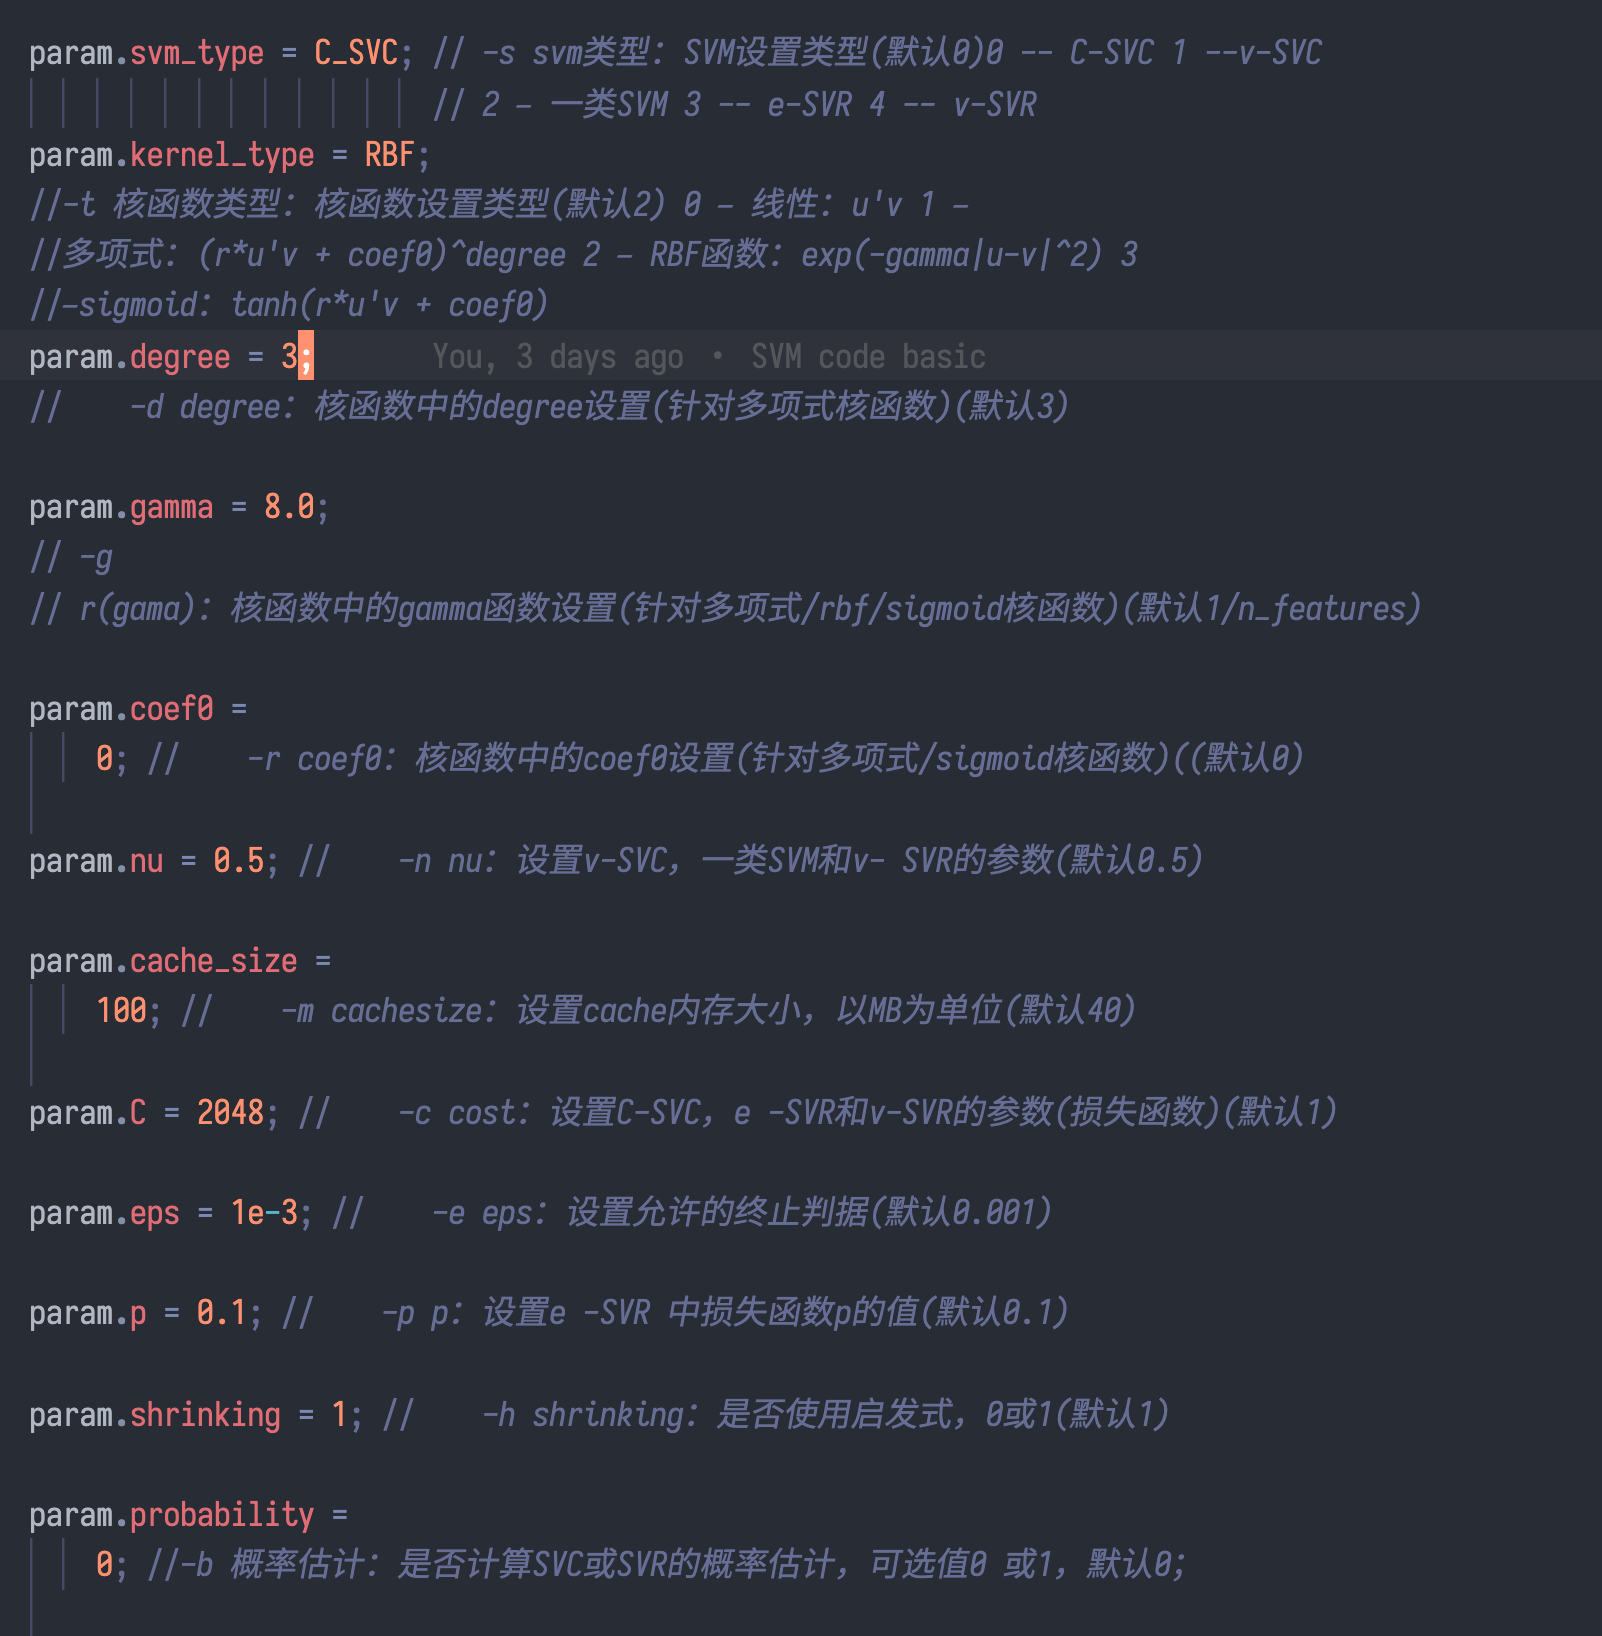
\includegraphics[width=0.5\textwidth]{image/d01-p}
    \caption{two-spiral problem-parameter}
  \end{figure}
  \begin{figure}[H]
    \centering
    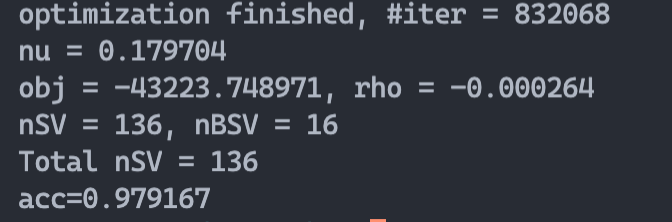
\includegraphics[width=0.5\textwidth]{image/d01}
    \caption{two-spiral problem-output}
  \end{figure}
  

  \subsection{Data2}
  \textbf{Test Data}

  We set the former 3677 samples as training set, the latter 500 samples as test set.  
  
  \textbf{Classifier}

  The \textbf{ Abalone Age Problem} is regression problem.
  In this dataset, I applied Epsilon-SVR.

  \textbf{Parameter}

  SVM Type: Epsilon-SVR

  Kernel: RBF

  Cost: 4

  C is the penalty coefficient, that is, tolerance for errors. The higher the c, the more intolerable the error is, and it is easy to overfit. The smaller C, the easier to underfit. C is too large or too small, the generalization ability becomes poor


  gamma: 1

  Gamma is a parameter that comes with this function after selecting the RBF function as the kernel. It implicitly determines the distribution of the data after mapping into a new feature space. For gamma replacement, the fewer support vectors, the smaller the gamma value and the more support vectors. The number of support vectors affects the speed of training and prediction.


  \begin{figure}[H]
    \centering
    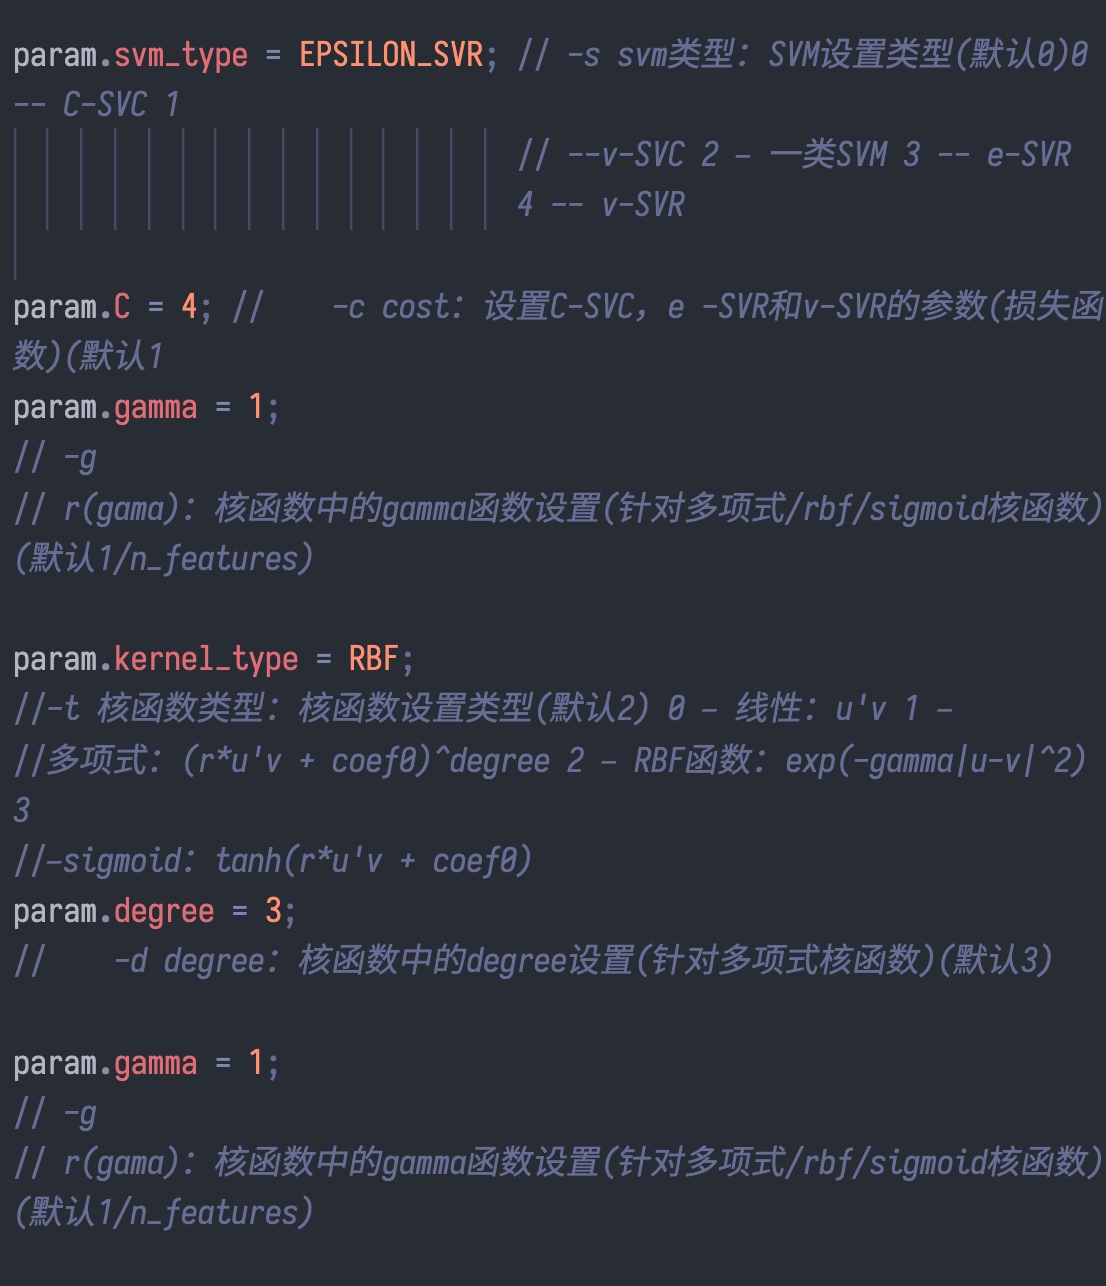
\includegraphics[width=0.3\textwidth]{image/d02}
    \caption{Abalone Age Problem parameter}
  \end{figure}

  \textbf{Accuracy}
  acc=0.706
  
  \textbf{Output}


  \begin{figure}[H]
    \centering
    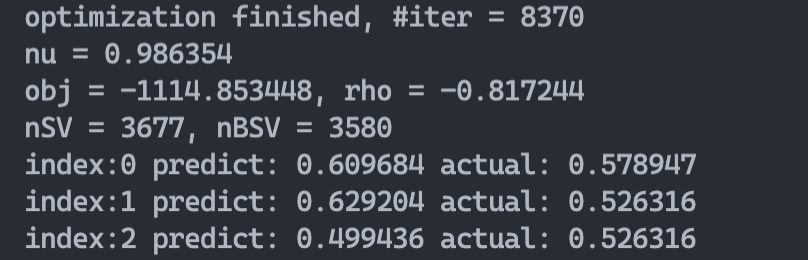
\includegraphics[width=0.5\textwidth]{image/d021}
    \caption{Abalone Age Problem parameter}
  \end{figure}

  \begin{figure}[H]
    \centering
    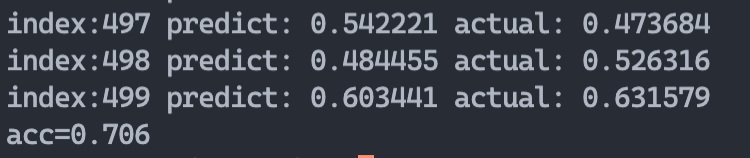
\includegraphics[width=0.5\textwidth]{image/d022}
    \caption{Abalone Age Problem parameter}
  \end{figure}
  
  \textbf{Tuning}

  It should be noted that the physical meaning of gamma. We mentioned that the width of many RBFs will affect the range of Gaussian corresponding to each support vector, thereby affecting the generalization performance. My understanding: If the gamma is set too large, the variance will be small, and the Gaussian distribution with small variance will be tall and thin, which will only act near the support vector samples, and it has a poor classification effect for unknown samples. There is training The accuracy rate can be very high, (if the variance is infinitesimally small, theoretically, the SVM of the Gaussian kernel can fit any nonlinear data, but it is easy to overfit) and the possibility that the test accuracy rate is not high is usually overtraining; If the setting is too small, the smoothing effect will be too large to obtain a particularly high accuracy rate on the training set, and it will also affect the accuracy rate of the test set.

  \subsection{Data3}

  \textbf{Test Data}
 
  There are 349 samples, first 299 as training data, last 50 as training data.

  \textbf{Classifier}

  C-SVC and RBF as kernel function. The penalty coefficient C is the coefficient of the slack variable that we talked about in the previous chapter. In the optimization function, it mainly balances the relationship between the complexity of the model and the misclassification rate, which can be understood as the regularization coefficient. When C is larger, our loss function will also be larger, which means that we are reluctant to give up farther outliers. In this way, we will have fewer support vectors, which means that the support vector and hyperplane models will become more complicated and easy to overfit. On the contrary, when C is relatively small, it means that we do n’t want to deal with those outliers and will choose more samples as support vectors. The final support vectors and hyperplane models will also be simple. 

  Another hyperparameter is the parameter gamma of the RBF kernel function. gamma mainly defines the influence of a single sample on the entire classification hyperplane. When gamma is relatively small, the influence distance of a single sample on the entire classification hyperplane is relatively long, and it is easy to be selected as a support vector. On the contrary, when gamma is relatively large, a single sample affects the entire The influence distance of the classification hyperplane is relatively short, and it is not easy to be selected as the support vector, or the support vector of the entire model will be less, and the model will become more complicated.


  \textbf{Parameter}

  C = 2

  gamma = 2

  \textbf{PrintOut}

  \begin{figure}[H]
    \centering
    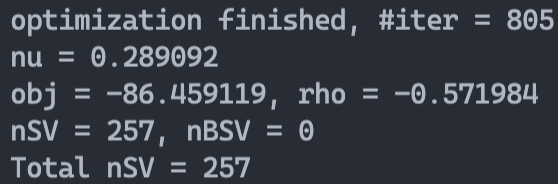
\includegraphics[width=0.5\textwidth]{image/d03}
    \caption{SPECT Heart Diagnosis Problem}
  \end{figure}

  \begin{figure}[H]
    \centering
    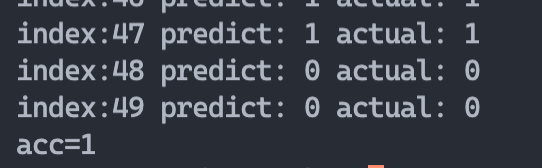
\includegraphics[width=0.5\textwidth]{image/d03o}
    \caption{SPECT Heart Diagnosis Problem}
  \end{figure}
\end{homeworkProblem}

\begin{homeworkProblem}
  \subsection{Steps}
  \begin{enumerate}
    \item Initialize various variables: read datafile, set parameter
    \item Initialize population: gene is the visiting order, each individual is one visiting order.
    \item Implement Fitness function: $f=1/distance$
    \item Implement Select function: Roulette 
    \item Implement Crossover function: crossover visiting order by Probability $P_m$, keep the first and the last one city, reorder the middle ones.
    \item Implement Mutation function: Randomly mutate 2 point of the visiting order
    \item Implement main loop 
  \end{enumerate}

  \subsection{Detail}
  \begin{enumerate}
    \item Encoding method: The general encoding methods are binary encoding method, Gray code encoding method, floating point encoding method, symbol encoding method, and real number encoding used directly this time
    \item Group composition: Elite retention
    There are four ways to form a new generation group composition method:
    \begin{itemize}
      \item N: all-new-generation inter-generational updates that replace the previous generation groups
      \item G: update the partial update method of some individuals in the group according to a certain proportion (or generation gap method, the extreme of this case is to delete only the worst way of death for each uncomfortable individual).
      \item E: The best retention (elitist) group construction method that keeps a best parent string.
      Method.
      \item B: Select the best group formation form of the individual from the children and parents.
      Generally speaking, the global search performance of N mode is the best, but the convergence speed is the slowest; the convergence speed of B mode is the fastest, but the global search performance is the worst; the performance of E mode and G mode is between N mode and B mode. In the application of the solution to the salesman problem, the E method is mostly used.

    \end{itemize}
    For performance considerations, the E method was adopted in this comprehensive training. In the selection of the first generation, the selection crossover and mutation of each generation used the ideas retained by the elite.    
  \end{enumerate}
  How can we allow more elite individuals to survive, and still maintain the richness of the guaranteed species, thereby reducing more algorithm running time?
  We first divide the group into two different groups, that is, to survive in two regions with different environments to form geographical isolation. The purpose of this is to increase the richness of the population. After that, we changed the living environment of two different groups into evil strategies (that is, two different and more demanding and complex selection criteria). The purpose of this is to allow more elite individuals to survive. When the two populations have multiplied to a certain standard, they will be merged into a single population, and eventually a global optimal solution will be generated more quickly through a certain standard.

  \subsection{Train}
  \begin{figure}[H]
    \centering
    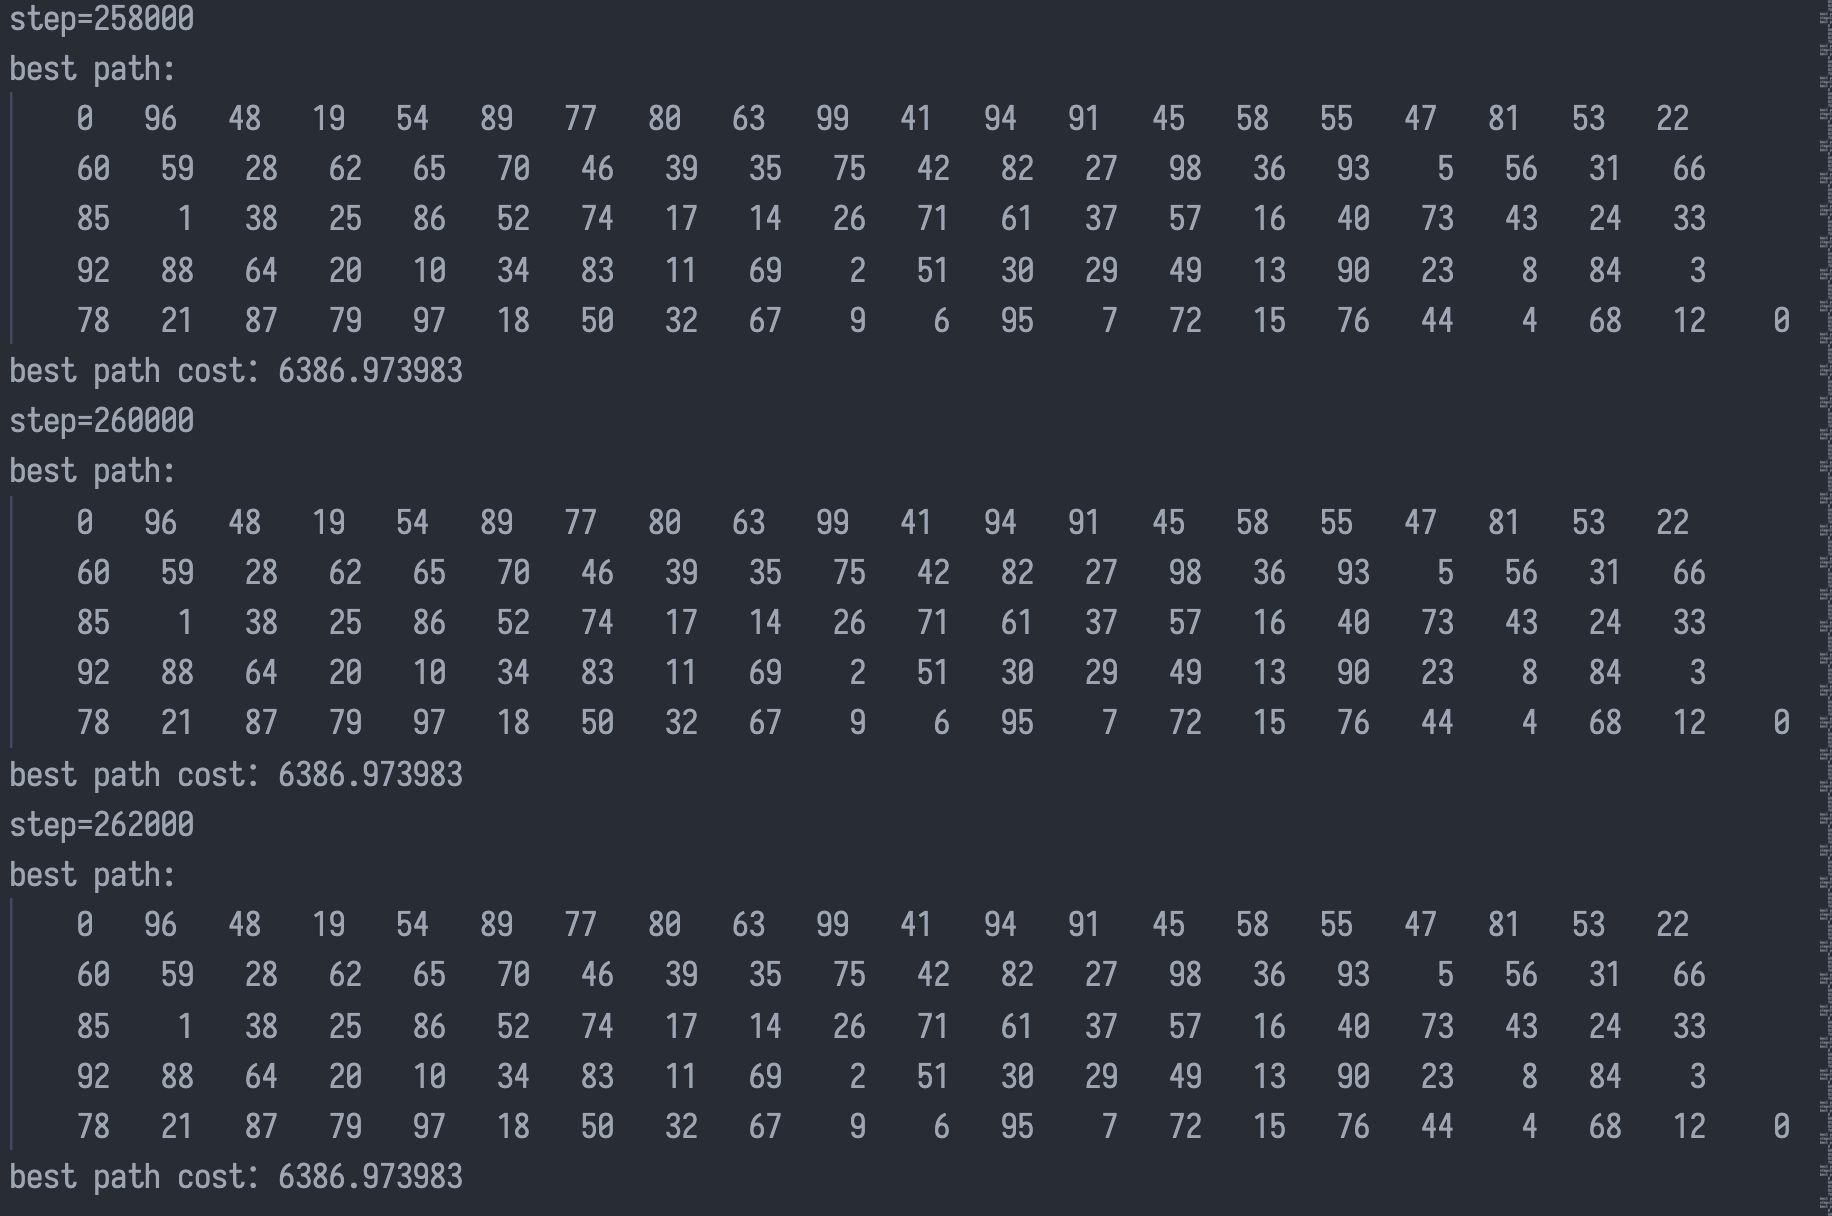
\includegraphics[width=0.5\textwidth]{image/path100}
    \caption{The Training Outcome (100 citys)}
  \end{figure}
  \begin{figure}[H]
    \centering
    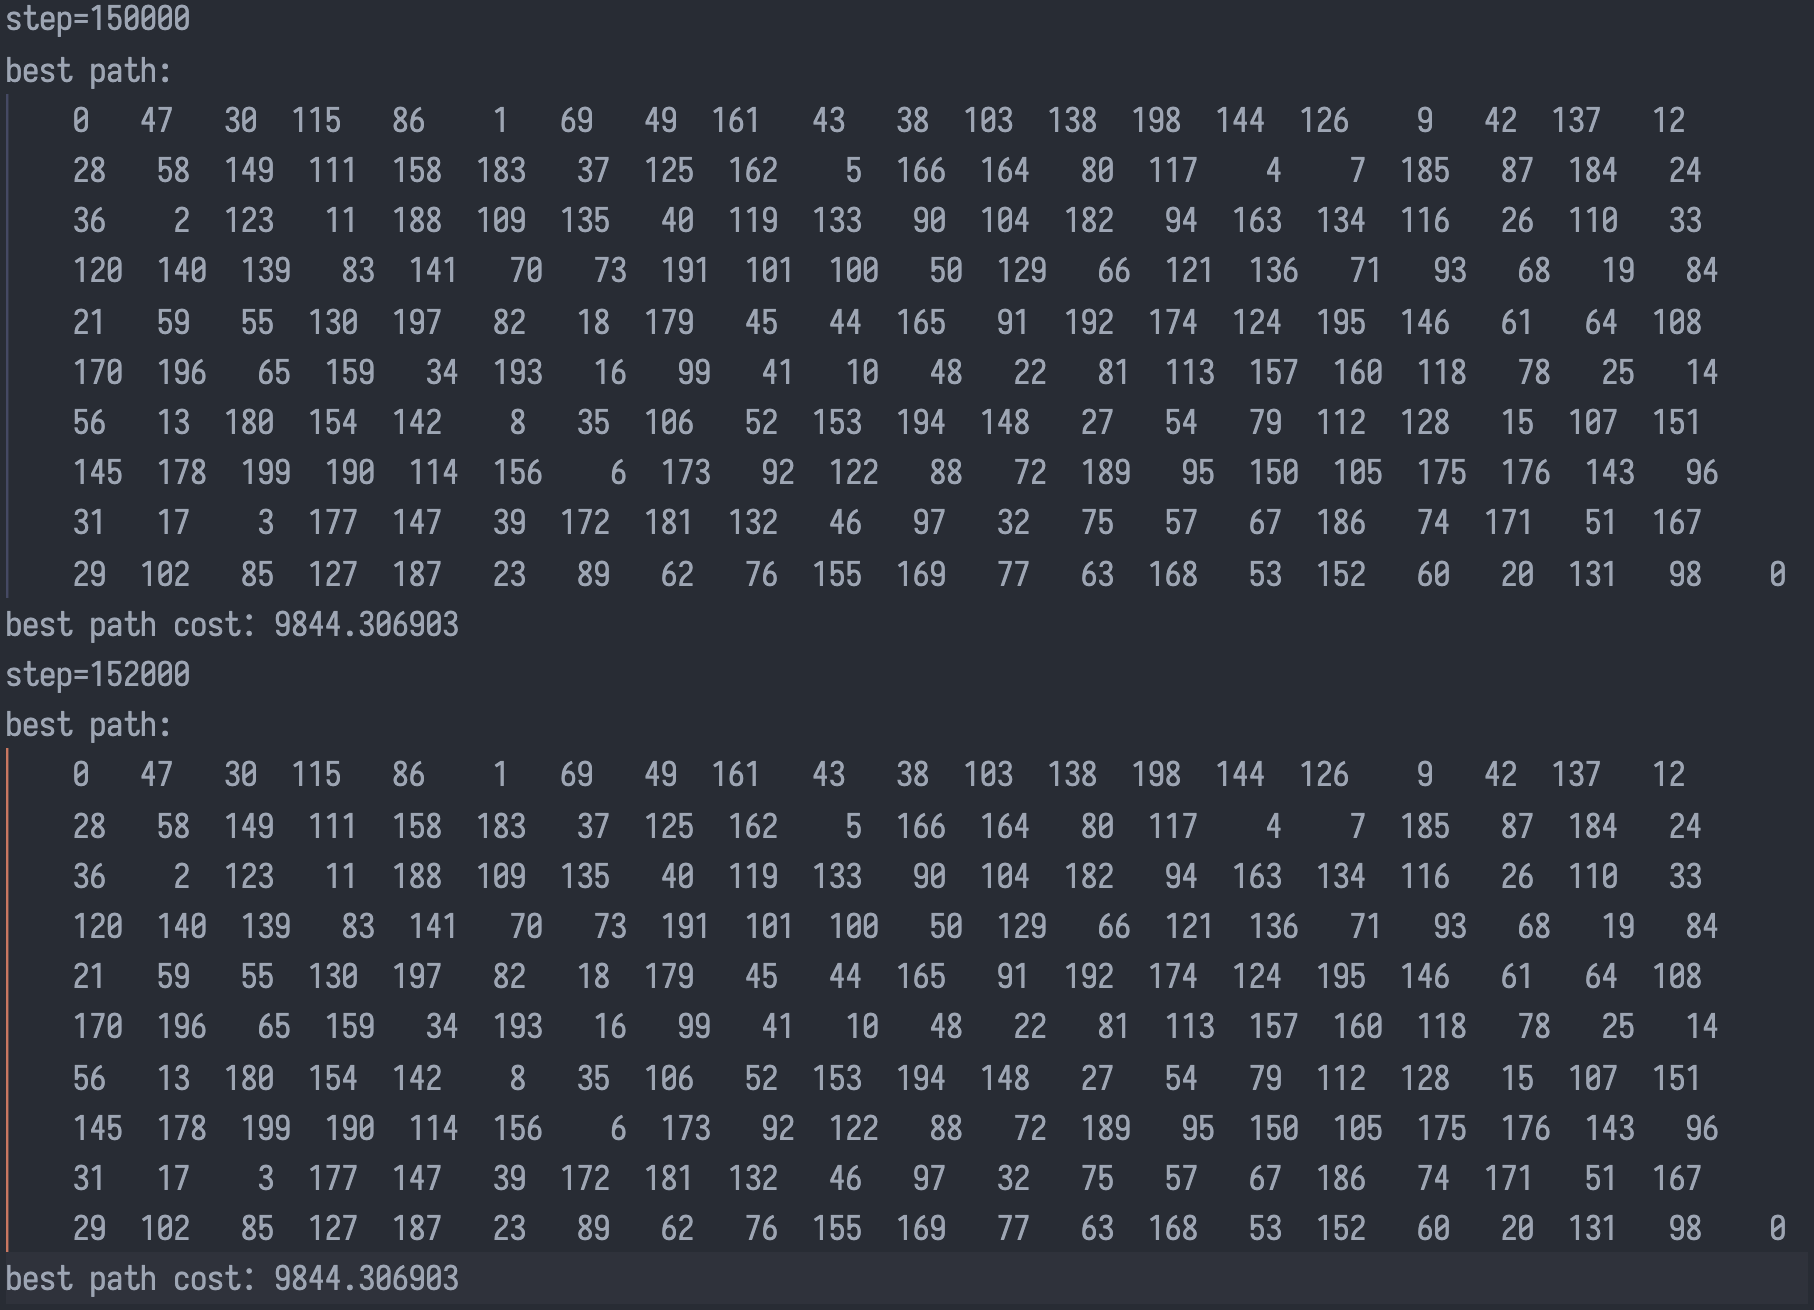
\includegraphics[width=0.5\textwidth]{image/path200}
    \caption{The Training Outcome (200 citys)}
  \end{figure}
  \begin{figure}[H]
    \centering
    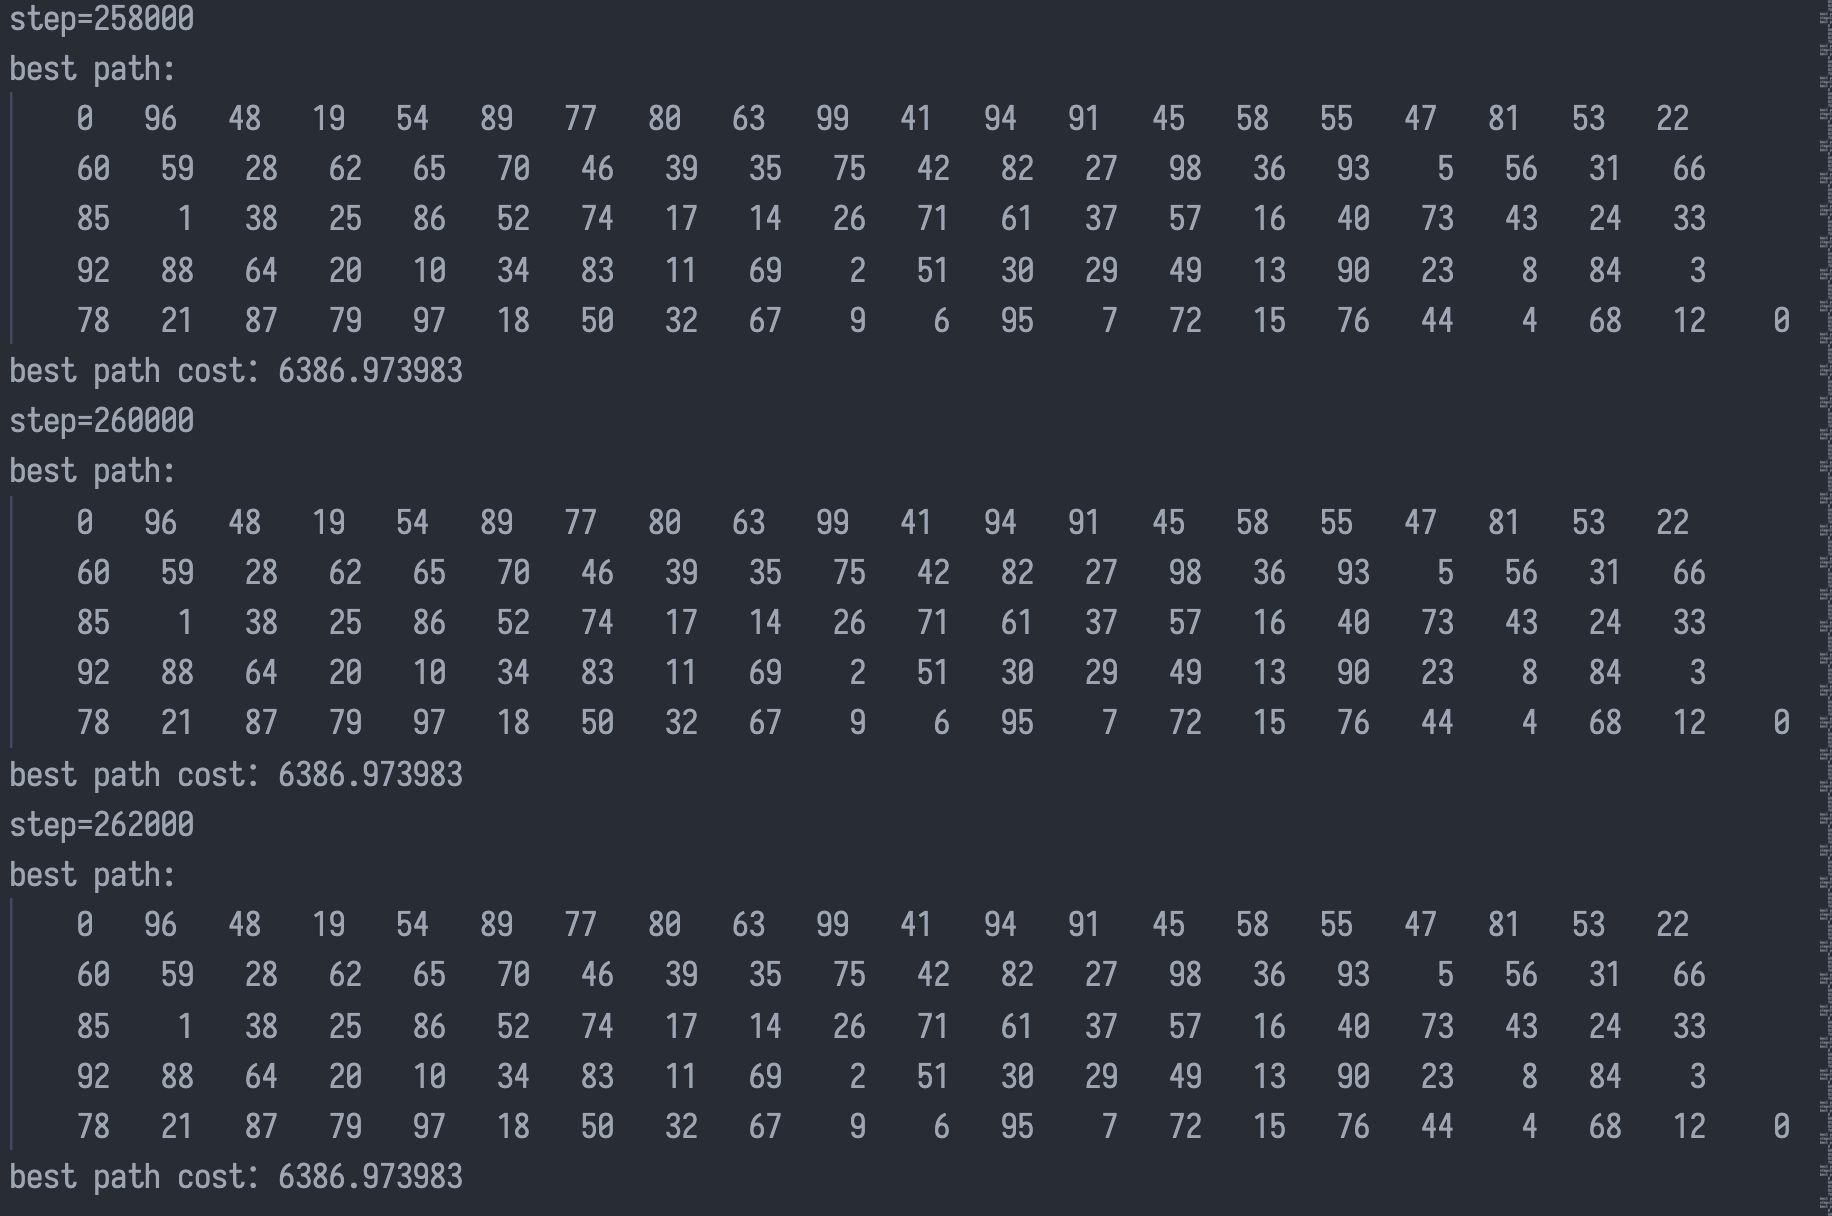
\includegraphics[width=0.5\textwidth]{image/path100}
    \caption{The Training Outcome (300 citys)}
  \end{figure}
  \begin{figure}[H]
    \centering
    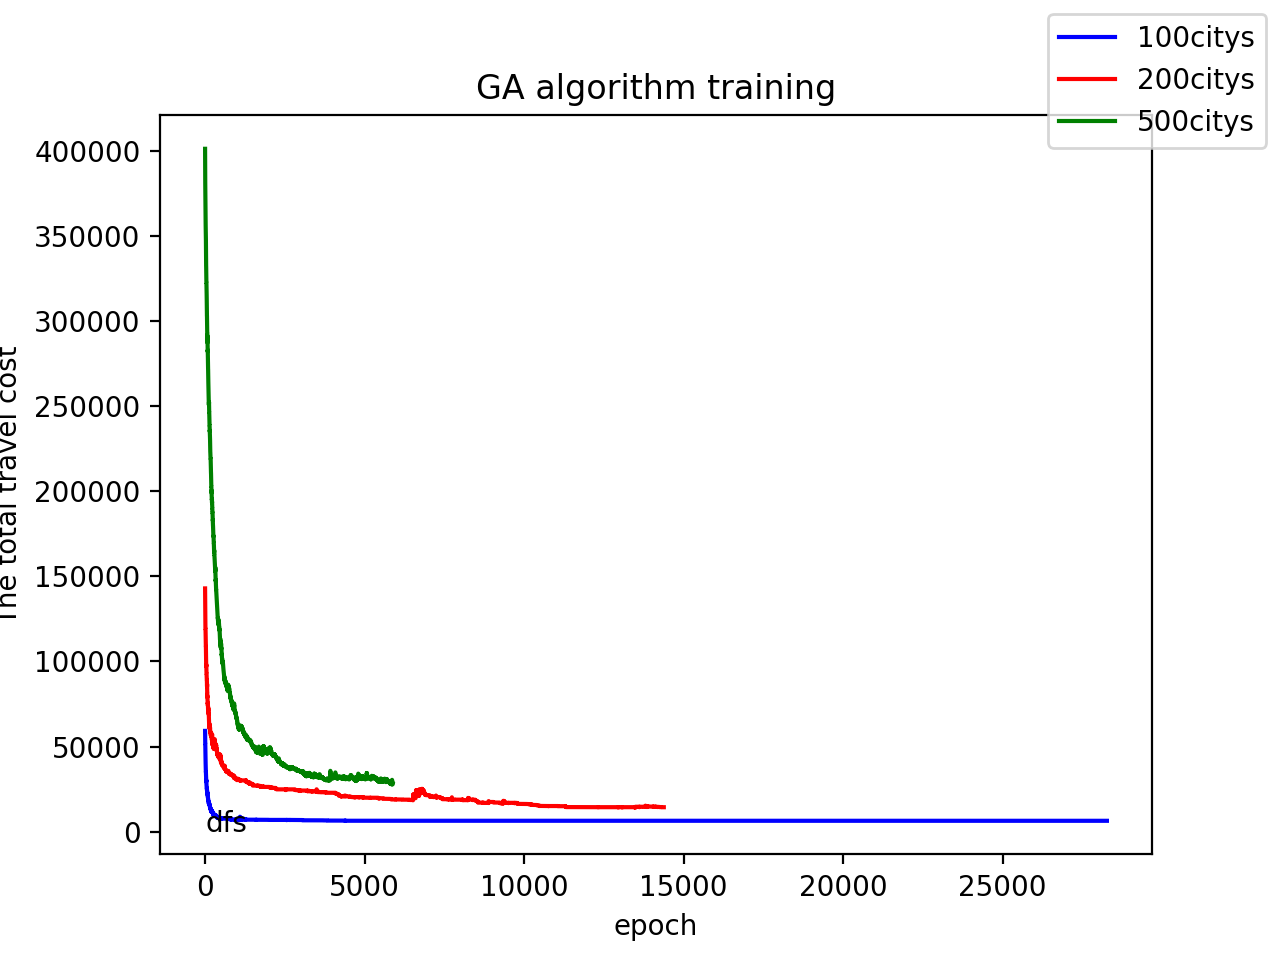
\includegraphics[width=0.5\textwidth]{image/train}
    \caption{The Training Convergence}
  \end{figure}
\end{homeworkProblem}
\end{document}
